\subsection{Calorimeters}

The calorimeters are designed to measure the energy from particles by absorbing them.
They are located outside the solenoidal magnet that surrounds the inner detector.
The ATLAS calorimeters are comprised of a number of sampling calorimeters with full $\phi$-symmetry and the pseudorapidity range of $|\eta|<4.9$.
Figure~\ref{fig:calo_dec} shows the layout of the ATLAS calorimeter system.
As mentioned in overview section, there are two basic calorimeter systems: an inner electromagnetic (EM) calorimeter and an outer hadronic calorimeter.
The EM calorimeter is designed for precise measurements for electrons and photons, so that with fine granularity;
while the hardronic one with relative coarser granularity but satisfied the physics requirements for jets reconstructions and $E_{T}^{miss}$ measurements.
Two different sampling techniques are used, the EM calorimeter is purely based on liquid-argon (LAr) technology, hardronic calorimeter use both LAr and scintillating tiles calorimeters. 
More details are described as belows.
\begin{figure}[!htb]
  \centering
  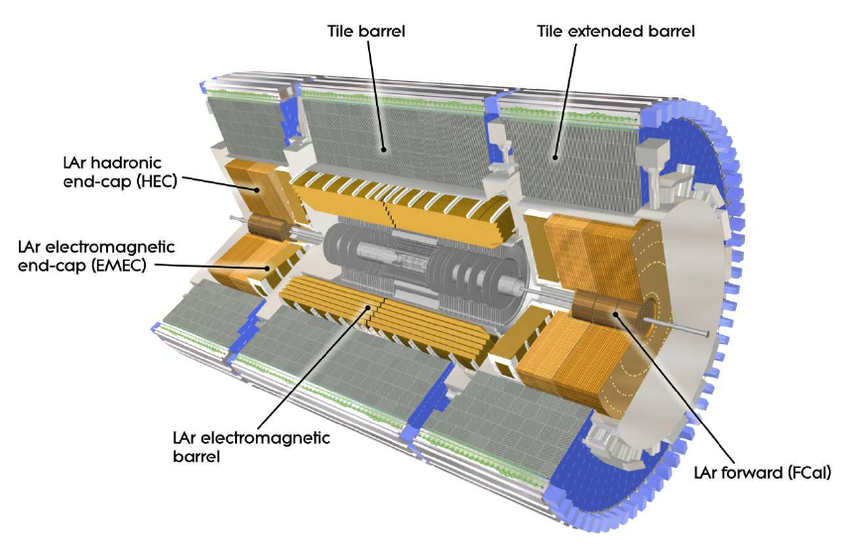
\includegraphics[width=0.8\textwidth]{figures/Detector/calo_layout.png}
  \caption{Cut-away view of the ATLAS calorimeters. The LAr calorimeters are seen inside the scintillator- based Tile hadronic calorimeters\cite{Buchanan:2008}.}
  \label{fig:calo_dec}
\end{figure}

%% ================================ LAr calorimeter ===================
\textbf{Liquid Argon calorimeter}

The LAr calorimeter is the one uses liquid-argon as active medium.
The Liquid Argon sampling calorimeter technique with "accordion-shaped" electrodes is used for all electromagnetic calorimetry covering the pseudorapidity range of $|\eta|<3.2$;
and for hadronic calorimetry from $|\eta| = 1.4$ up to the acceptance limit $|\eta| = 4.9$\cite{CERN-LHCC-96-041}.
Figure~\ref{fig:calo_lar} shows the shape of a barrel module as accordion geometry.
For barrel EM calorimeter, the absorbing material is lead-liquid argon, while the hadronic end-cap calorimeter use copper plates as the absorbing material.
In addition, the forward calorimeter is splited into three parts, an EM sector in which copper is used as absorbing material and two hadronic sectors using tungsten ouside the EM sector.
\begin{figure}[!htb]
  \centering
  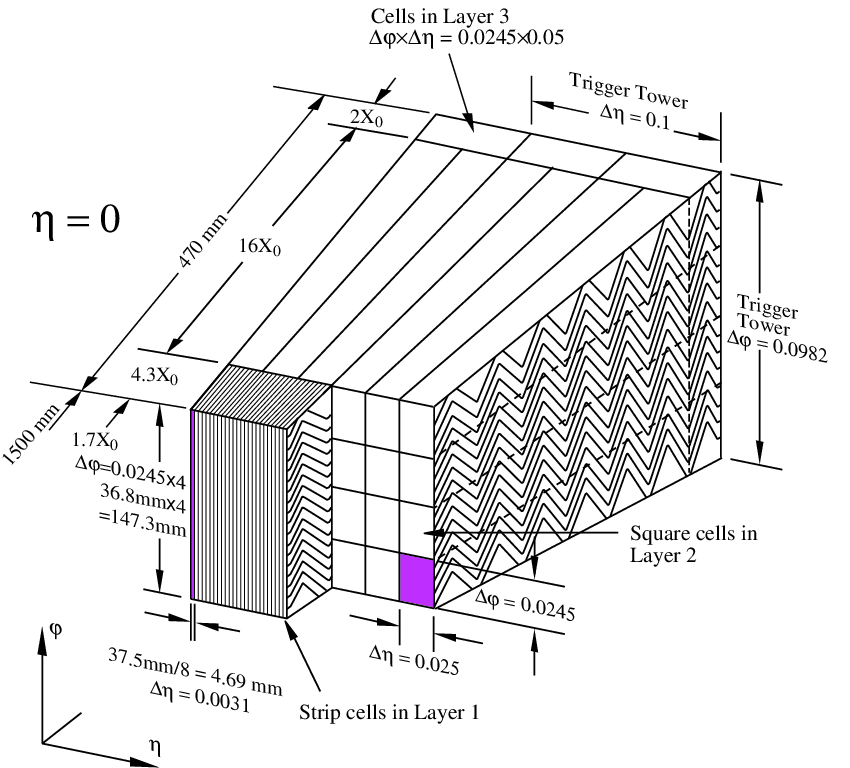
\includegraphics[width=0.6\textwidth]{figures/Detector/calo_lar.png}
  \caption{Schematic diagram of a LAr EM calorimeter barrel module.}
  \label{fig:calo_lar}
\end{figure}

%% =============================== Tile calorimeter ====================
\textbf{Tile calorimeter}

Tile calorimeter is a sampling calorimeter that use scintillating plates as active medium and steel as absorber.
It consists of three sections: the central barrel with the pseudorapidity range of $|\eta|<1.0$ and two extended barrels with $0.8 < |\eta| < 1.7$.
Figure~\ref{fig:calo_tile} shows the design of one tile calorimeter module.
It's used for energy reconstruction of jets and $E_{T}^{miss}$ measurement by combining with the forward and end-cap hadronic calorimeter.
\begin{figure}[!htb]
  \centering
  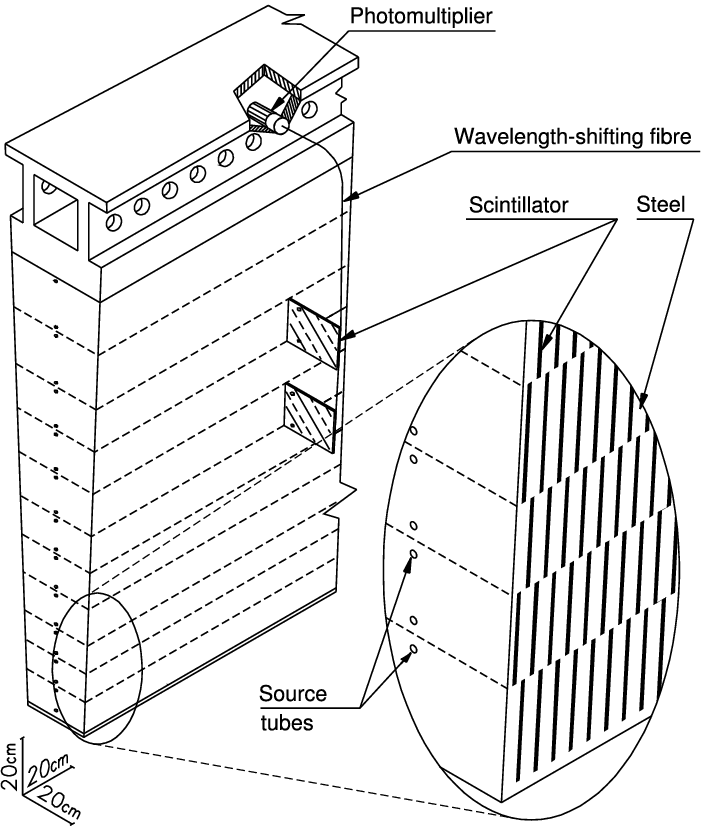
\includegraphics[width=0.5\textwidth]{figures/Detector/calo_tile.png}
  \caption{Schematic diagram of tile calorimeter module\cite{Aad:2010}.}
  \label{fig:calo_tile}
\end{figure}

